\documentclass[UTF8]{ctexart}
%\documentclass{article}
\usepackage{graphicx,amsfonts,amsmath,mathrsfs,amssymb,amsthm,url,color}
\usepackage{fancyhdr,indentfirst,bm,enumerate,natbib, float,tikz,graphicx}
\usepackage{caption}
\usepackage{subcaption}
\title{2025春《实用随机过程》期末考试卷}
\author{}
\date{}
\textheight 23cm
 \textwidth 16.5cm
  \topmargin -1.2cm
   \oddsidemargin 0cm
    \evensidemargin 0cm

\begin{document}
\maketitle




\noindent 一、(12分) 设离散时间 Markov 链 $\{X_n, n = 0,1,2,\ldots\}$ 的状态空间为 $\{1,2,3,4\}$,且转移概率矩阵为
\[
\begin{pmatrix}
1 & 0 & 0 & 0 \\
0.2 & 0.3 & 0.5 & 0 \\
0 & 0.6 & 0.4 & 0 \\
0 & 0 & 0 & 1
\end{pmatrix}
\]
(1) 指出该 Markov 链有几个类,并写出每个类所包含的状态。\\
(2) 记 $T = \min\{n \geq 0 : X_n =  \text{1 或 4} \}$,试求 $\mathbb{E}[T|X_0 = 2]$。\\
解:(1)一共有三个类,分别为$\{1\};\{2,3\};\{4\}$(状态1和4都是吸收态)\\
(2)注意从状态2开始不可能到达状态4,$T = \min\{n \geq 0 : X_n = 1\}$,记
\[
\mathbb{E}[T|X_0 = 2]=T_2\quad
\mathbb{E}[T|X_0 = 1]=T_1\quad
\mathbb{E}[T|X_0 = 0]=T_0=0
\]
对从初始状态2的第一次转移取条件(注意至少要转移一次才能到达状态1):
$$
\begin{aligned}
	T_2 &= 1+0.3T_2+0.5T_3 \\
	T_3 &= 1+0.6T_2+0.4T_3
\end{aligned}
$$
有
\[
T_2=\frac{55}{6} \quad T_3=\frac{65}{6}
\]
即$\mathbb{E}[T|X_0 = 2]=\frac{55}{6}$\\


\noindent 二、(30分) 设有一个质点在如原所示的二叉树上(共 $m = 3$ 层)作随机游走。它从顶点 0 出发,每隔单位时间等概率沿边转移到某个邻点上。以 $X_n$ 表示该质点所在顶点的编号,则 $\{X_n, n \geq 0\}$ 为一 Markov 链。
\begin{figure}[h!]
\centering
	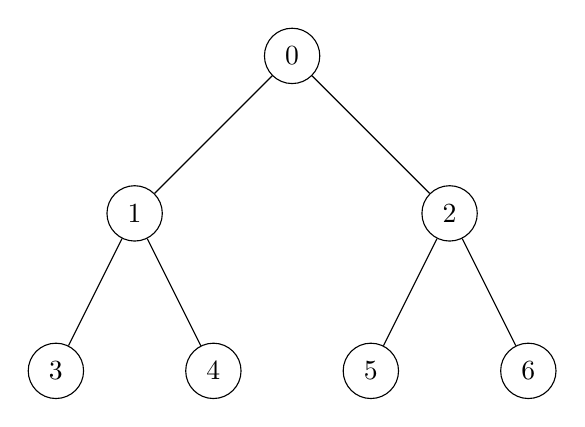
\begin{tikzpicture}
		\tikzset{
		box/.style ={
		circle, %圆形节点
		minimum width =20pt, %最小宽度
		minimum height =20pt, %最小高度
		inner sep=3pt, %文字和边框的距离
		draw=black, %边框颜色
		fill=white
		}
		}
		\node[box] (1) at(0,0){0};
		\node[box] (2) at(-2,-2){1};
		\node[box] (3) at(2,-2){2};
		\node[box] (4) at(-3,-4) {3};
		\node[box] (5) at(-1,-4){4};
		\node[box] (6) at(1,-4){5};
		\node[box] (7) at(3,-4){6};
		\draw[-] (1)--(2);
		\draw[-] (1)--(3);
		\draw[-] (2)--(4);
		\draw[-] (2)--(5);
		\draw[-] (3)--(6);
		\draw[-] (3)--(7);
	\end{tikzpicture}
\end{figure}

\noindent (1) 试写出该Markov链的一步转移概率矩阵 \( \bm{P}_3 \)。\\
(2)对任意顶点 \( i \) (\( 0 \leq i \leq 6 \)),讨论其周期性和常返性。\\
(3)对任意顶点 \( i \) (\( 0 \leq i \leq 6 \)),求质点从 \( i \) 出发后首次返回 \( i \) 所需平均步数 \( \mu_i \)。\\
(4) 在稳态条件下,该Markov链是否时间可逆?需说明理由。\\
(5) 对一般的 \( m \) (\( m \geq 1 \)),试求该Markov链的平稳分布(可不写计算过程)。\\
解:(1)一步转移概率矩阵为
\[
\bm{P}_3=
\begin{pmatrix}
	0 & \frac{1}{2} &\frac{1}{2} & 0 &0 &0&0\\
	\frac{1}{3} & 0&0 & \frac{1}{3} &\frac{1}{3} &0&0\\
	\frac{1}{3} & 0&0 & 0 &0 &\frac{1}{3}&\frac{1}{3}\\
	0 & 1 &0 & 0 &0 &0&0\\
	0 & 1 &0 & 0 &0 &0&0\\
	0 & 0&1 & 0 &0 &0&0\\
	0 & 0&1 & 0 &0 &0&0\\
\end{pmatrix}
\]
(2)所有状态互通,对于每个状态至少需要两步回到自身,则所有的状态的周期为2\\
又Markov链是不可约有限状态的,则所有状态都是正常返的\\
(3)利用有限加权边图上的随机游走的结论,对存在的每条边赋权重$w_{ij}=1$,就满足上述转移概率矩阵,且有\\
\[
\sum\limits_{i,j}^{} w_{ij}=12
\]
上式是因为每条边(共6条)要计数两遍(这样比单独计数每个状态的边之后再相加来的方便)\\
\[
\pi_i=\frac{\sum\limits_{j}^{} w_{ij}}{\sum\limits_{i,j}^{} w_{ij}}
\]
\[
\pi_i=
\begin{cases}
	\frac{1}{6}  &  i=0 \\
	\frac{1}{4} &  i=1,2\\
	\frac{1}{12} & i=3,4,5,6
\end{cases}
\]
\[
\mu_i=\frac{1}{\pi_i}=
\begin{cases}
	6  &  i=0 \\
4 &  i=1,2\\
12 & i=3,4,5,6
\end{cases}
\]
(4)当然可逆,这是有限加权边图上的随机游走的结论之一\\
可以代入平稳方程一一验证:\\
\[
\pi_i=\sum\limits_{j}^{} \pi_j P_{ji}
\]
(5)类似(3),仍然对存在的边赋权重$w_{ij}=1$\\
\[
\sum\limits_{i,j}^{} w_{ij}=2(2+\dots+2^{m-1})=2^{m+1}-4
\]
第一层的点连接2个边,最后一层的点连接1个边,其余的点连接3个边,则\\
\[
\pi_i=
\begin{cases}
	\frac{1}{2^m-2}  &  i=0 \\
	\frac{1}{2^{m+1}-4} &  \text{i在第m层}\\
	\frac{3}{2^{m+1}-4} & \text{其他}
\end{cases}
\]\\


\noindent 三、(16分) 设连续时间 Markov 链 $\{X(t), t \geq 0\}$ 的状态空间为 $\{1,2,3\}$,且其 $Q$ 矩阵为
\[
Q = 
\begin{pmatrix}
-2 & 1 & 1 \\
0 & -3 & 3 \\
2 & 0 & -2
\end{pmatrix}
\]
(1) 求对应嵌入链的转移概率矩阵。\\
(2) 当 $t \to \infty$ 时,求 $X(t)$ 的极限分布。\\
解:(1) $Q$ 矩阵指的是对角元为$-v_i$,非对角元为$q_{ij}$的矩阵\\
嵌入链的转移概率矩阵为:
\[
P=
\begin{pmatrix}
	0 & \frac{1}{2} & \frac{1}{2} \\
	0 & 0 & 1 \\
	1 & 0 & 0
\end{pmatrix}
\]
(2)设连续链的极限概率$P_i$,有方程(总离开速率等于总进入速率):\\
$$
\begin{aligned}
	 2P_1& =2P_3 \\
	3P_2 & =P_1\\
	2P_3&=P_1+3P_2
\end{aligned}
$$
\[
P_1+P_2+P_3=1
\]
有
\[
P_1=P_3=\frac{3}{7} \quad P_2=\frac{1}{7}
\]
也就是
\[
P(\lim_{t\rightarrow \infty} X(t)=1)=P(\lim_{t\rightarrow \infty} X(t)=3)=\frac{3}{7} \quad P(\lim_{t\rightarrow \infty} X(t)=2)=\frac{1}{7}
\]\\


\noindent 四、(10分) 设 $\{X(t), t \geq 0\}$ 为一个线性生灭过程,且生长率和死亡率分别为 $\lambda_n = n\lambda$ 和 $\mu_n = n\mu$, $n \geq 0$,其中 $\lambda, \mu > 0$ 为给定常数。如果初始状态 $X(0) = 1$,试求灭绝概率 $q= \lim_{t \to \infty} P(X(t) = 0|X(0) = 1)$。\\
解:\\
考虑分支过程,但要注意分支过程是Markov链而非连续链,设此连续链的嵌入链为$\{Y(t), t \geq 0\}$,有转移概率:\\
\[
P_{i,i+1}=\frac{\lambda}{\lambda+\mu} \quad P_{i,i-1}=\frac{\mu}{\lambda+\mu}
\]
同时
\[
\text{从一个个体开始的连续链最终灭绝} \iff \text{从一个个体开始的嵌入链最终灭绝}
\]
因此只需要求嵌入链的灭绝概率即可;注意分支过程的定义为第$t-1$代的每个父代独立产生的第$t$代子代的总数量(相当于父代产生子代之后死亡),而本题父代在产生子代之后还存活,把本题存活的父代看成他自己产生的子代,同时认为父代产生子代之后死亡,记一个父代产生$i$个子代的概率为$P_i$,同时定义:\\
\[
\{\tilde{Y}(t):\tilde{Y}(0)=1\quad \tilde{Y}(t)=Y\left(\sum\limits_{i=0}^{t-1}  \tilde{Y}(i) \right)  \quad t \geq 0\}
\]
则$\{\tilde{Y}(t) \}$为分支过程(相当于分支过程的父代为$Y(t)=n$时,我们认为下一代为$Y(t+n)$)\\
且有:
\[
q= \lim_{t \to \infty} P(Y(t) = 0|Y(0) = 1)= \lim_{t \to \infty} P(\tilde{Y}(t) = 0|\tilde{Y}(0) = 1)
\]
\[
P_0=\frac{\mu}{\lambda+\mu} \quad P_2=\frac{\lambda}{\lambda+\mu}
\]
利用分支过程定理有:
\[
q=P_0+P_2q^2
\]
注意$q$是满足上面方程的最小解:
\[
q=
\begin{cases}
	\frac{\mu}{\lambda}  & \frac{\mu}{\lambda}<1  \\
	1  &  \frac{\mu}{\lambda}\ge 1
\end{cases}
\]
另解:\\
记$q_2=\lim_{t \to \infty} P(X(t) = 0|X(0) = 2)$,对第一次转移取条件\\
\[
q=\frac{\mu}{\lambda+\mu}+\frac{\lambda}{\lambda+\mu}q_2
\]
而从状态2开始的嵌入链如果想灭绝的话,必须先到达1,再从1到达0;在到达1之前可以视1为一个“暂时的”吸收壁,那么可以看到这时从2开始的嵌入链(带有吸收壁1)和从1开始的嵌入链具有相同的性质(它们的转移概率矩阵一样),所以从2“灭绝到”1的概率也是$q$,当到达状态1之后我们认为这个吸收壁被取消了,此时从状态1到达状态0的概率就是$q$,即$q_2=q^2$,得到相同的方程(写到这里也不难发现这其实就是分支过程的方程了)\\

\noindent 五、(14分) 设 $\{B(t), t \geq 0\}$ 为标准 Brown 运动。\\
(1)试求随机变量 $X = B(1) + B(2) + B(3)$ 的分布。\\
(2) 在给定 $B(2) = 1$ 的条件下,试求 $B(1)$ 和 $B(3) + B(4)$ 的联合分布。\\
解:(1)利用独立增量性和平稳增量性:\\
\[
X=3B(1)+2(B(2)-B(1))+(B(3)-B(2))
\]
\[
B(1),B(2)-B(1),B(3)-B(2) \sim N(0,1) \quad \text{且相互独立}
\]
则
\[
X \sim N(0,14)
\]
(2)
\[
B(1)|B(2)=1 \sim N\left(\frac{1}{2},\frac{1}{2}\right)
\]
另一方面$B(3)+B(4)=2B(3)+(B(4)-B(3))$,又
\[
B(3)|B(2)=1 \sim B(2)+(B(3)-B(2))|B(2)=1\sim 1+N(0,1) \sim N(1,1)
\]
\[
B(4)-B(3)|B(2)=1\sim B(4)-B(3)\sim N(0,1)
\]
则
\[
B(3)+B(4)|B(2)=1 \sim N(2,5)
\]
注意Brown运动是Guass过程以及独立增量性($B(1)|B(2)=1$与$B(3)+B(4)|B(2)=1$独立),$(B(1),B(3)+B(4))|B(2)=1$是二元正态分布
\[
(B(1),B(3)+B(4))|B(2)=1 \sim N\left( \left( \frac{1}{2},2\right),
\begin{pmatrix}
	\frac{1}{2} & 0\\
	0& 5
\end{pmatrix}
 \right) 
\]
\textbf{RK}:\\
给定$B(t_1)=A,B(t_2)=B$的条件下,对$t_1<s<t_2$,$B(s)$的条件分布为$N\left(A+\frac{(B-A)(s-t_1)}{t_2-t_1},\frac{(s-t_1)(t_2-s)}{t_2-t_1}\right)$\\


\noindent 六、(18分) 考虑一质点在直线上从正整数 $a$ 出发的简单对称随机游走,其中 $0$ 和 $K(K > a)$ 为两个吸收态。设 $S_n$ 表示时刻 $n$ 该质点的位置,$S_0 = a$,而 $T = \min\{n : S_n = 0 \text{ 或 } K\}$,记
\[
M_n = \sum_{k=0}^n S_k - \frac{1}{3} S_n^3
\]
(1) 证明 $\{M_n, n \geq 0\}$ 为鞅。\\
(2) 试利用停时定理来求解 $\mathbb{E}[\sum_{k=0}^TS_k]$。\\
解:(1)利用$\mathbb{E}[X|U]=\mathbb{E}[\mathbb{E}[X|U,V]|U]$,并注意$S_1,\dots,S_n$实际上包含了$M_1,\dots,M_n$的所有信息\\
$$
\begin{aligned}
	\mathbb{E}[M_{n+1}|M_1,...,M_n] &= \mathbb{E}[\mathbb{E}[M_{n+1}|S_1,...,S_n]|M_1,...,M_n] \\
\end{aligned}
$$
其中
$$
\begin{aligned}
	\mathbb{E}[M_{n+1}|S_1,...,S_n] & =\mathbb{E}\left[\sum\limits_{k=0}^{n} S_k +S_{n+1}-\frac{1}{3}\left( S_n+X_{n+1}\right) |S_1,...,S_n\right] \\
	&=\mathbb{E}\left[\sum\limits_{k=0}^{n} S_k +S_{n}+X_{n+1}-\frac{1}{3}\left( S_n+X_{n+1}\right)|S_1,...,S_n \right]\\
	 & \stackrel{X_{n+1}\text{与}S_1,...,S_n\text{独立}}=\sum\limits_{k=0}^{n} S_k+S_n+\mathbb{E}[X_{n+1}]-\frac{1}{3}S_n^3-\frac{1}{3}\mathbb{E}[X_{n+1}^3]-S_n^2\mathbb{E}[X_{n+1}]-\mathbb{E}[X_{n+1}^2]S_n\\
	 &=\sum_{k=0}^n S_k - \frac{1}{3} S_n^3\\
	 &=M_n
\end{aligned}
$$
这就说明了
\[
	\mathbb{E}[M_{n+1}|M_1,...,M_n]=\mathbb{E}[\mathbb{E}[M_{n+1}|S_1,...,S_n]|M_1,...,M_n]=\mathbb{E}[M_n|M_1,...,M_n]=M_n
\]
另外
\[
\mathbb{E}[|M_n|]\le \mathbb{E}\left[\sum_{k=0}^n S_k  \right] +\frac{1}{3}\mathbb{E}[S_n^3] < \infty
\]
即$\{M_n, n \geq 0\}$ 为鞅\\
(2)先验证一下鞅停止定理的条件
$$
\begin{aligned}
	\mathbb{E}[|M_{n+1}-M_n|\mid M_1,...,M_n] & =\mathbb{E}\left[|S_{n+1}-\frac{1}{3}(S_{n+1}^3-S_n^3)|\mid M_1,...,M_n\right] \\
	 &   =\mathbb{E}\left[|S_{n+1}-\frac{1}{3}(X_{n+1}^3+3S_n^2X_{n+1}+3S_nX_{n+1}^2)|\mid M_1,...,M_n\right] \\
	 &\stackrel{\text{三角不等式}}<M
\end{aligned}
$$
则$$\mathbb{E}[M_T]=\mathbb{E}\left[ \sum_{k=0}^T S_k - \frac{1}{3} S_T^3\right] =\mathbb{E}[M_0]=a-\frac{1}{3}a^3$$\\
由赌徒破产模型(开始财富为$a$,公平赌模型下,财富先到达$K$而不是0的概率):
\[
P(S_T=K)=\frac{a}{K}
\]
\[
\mathbb{E}\left[S_T^3 \right] =P(S_T=K)K^3=aK^2
\]
最后
\[
\mathbb{E}\left[ \sum_{k=0}^TS_k\right] =\frac{1}{3}aK^2+a-\frac{1}{3}a^3
\]\\


\noindent 七、(附加题, 10分) 证明标准 Brown 运动 $\{B(t), t \geq 0\}$ 在任一区间 $[0,t]$ 上的二次变差为 $t$,即对区间 $[0,t]$ 上的任意分割 $0 = t_0 < t_1 < \cdots < t_n < t_{n+1} = t$,当 $n \to \infty$ 时,若最大间隔 $\max_{0 \leq i \leq n}(t_{i+1} - t_i) \to 0$,则有 $Q_n = \sum_{k=0}^n [B(t_{k+1}) - B(t_k)]^2$ 依概率收敛到 $t$。\\
解:证明依概率收敛$P(|Q_n-t|\ge \epsilon)\rightarrow0$考虑Markov不等式或者Chebyshev不等式\\
$$
\begin{aligned}
	\mathbb{E}[Q_n] & =\mathbb{E}\left[\sum_{k=0}^n [B(t_{k+1}) - B(t_k)]^2 \right]  \\
 & =\sum_{k=0}^n \mathbb{E}\left[ [B(t_{k+1}) - B(t_k)]^2\right] 
\end{aligned}
$$
另外
\[
B(t_{k+1})-B(t_k) \sim N(0,t_{k+1}-t_k) \quad \mathbb{E}\left[ [B(t_{k+1}) - B(t_k)]^2\right] =t_{k+1}-t_k
\]
则
\[
\mathbb{E}[Q_n]=\sum_{k=0}^n \mathbb{E}\left[ [B(t_{k+1}) - B(t_k)]^2\right] =t
\]
由独立增量性:
$$
\begin{aligned}
	\operatorname{Var}(Q_n) & =\operatorname{Var}\left(\sum_{k=0}^n [B(t_{k+1}) - B(t_k)]^2 \right)  \\
	& =\sum_{k=0}^n \operatorname{Var}\left( [B(t_{k+1}) - B(t_k)]^2\right)
\end{aligned}
$$
记$N_k=B(t_{k+1})-B(t_k) \sim N(0,t_{k+1}-t_k)$\\
$$
\begin{aligned}
	\operatorname{Var}(N_k)&=\mathbb{E}[N_k^4]-\left(\mathbb{E}[N_k^2] \right)^2\\
	& =3(t_{k+1}-t_k)^2-(t_{k+1}-t_k)^2\\
	& =2(t_{k+1}-t_k)^2
\end{aligned}
$$
利用Chebyshev不等式\\
$$
\begin{aligned}
	P(|Q_n-t|\ge \epsilon)&\le \frac{\operatorname{Var}(Q_n)}{\epsilon^2}\\
	&\le \frac{2\sum_{k=0}^n(t_{k+1}-t_k)^2}{\epsilon^2}\\
	&\le \frac{2\left( \sum_{k=0}^n(t_{k+1}-t_k)\right)\max\{
		t_{k+1}-t_k\}}{\epsilon^2}\\
		&\le \frac{2t\max\{
			t_{k+1}-t_k\}}{\epsilon^2}\\
			&\rightarrow 0
\end{aligned}
$$
这就说明了依概率收敛\\
\textbf{RK}:\\
对正态分布的高阶矩有
$$
\begin{aligned}
	X &\sim N(0,1)\\
	\forall k=2m>0&\quad \mathbb{E}[X^k]=(2m-1)!!
\end{aligned}
$$
也可以通过$N(\mu,\sigma^2)$的矩母函数$$M(t)=e^{\mu t+\frac{1}{2}\sigma^2t^2}$$或者特征函数$$\phi(t)=e^{i\mu t+\frac{1}{2}\sigma^2t^2}$$来获得高阶矩的信息\\
\end{document}